\documentclass[tikz,border=4pt]{standalone}
% Shared style for every figure and for the deck: one accent, one
% highlight, thin lines, rounded nodes, nothing decorative.
\usepackage[T1]{fontenc}
\usepackage{lmodern}
\renewcommand{\familydefault}{\sfdefault}
\usepackage{tikz}
\usetikzlibrary{arrows.meta,positioning,calc,shapes.misc,fit,backgrounds,decorations.pathreplacing}
\definecolor{ink}{RGB}{40,40,40}
\definecolor{soft}{RGB}{150,150,150}
\definecolor{faint}{RGB}{225,225,225}
\definecolor{accent}{RGB}{0,95,115}
\definecolor{accentlight}{RGB}{214,232,236}
\definecolor{warn}{RGB}{196,84,40}
\definecolor{warnlight}{RGB}{247,226,216}
\tikzset{
  every picture/.style={color=ink, line width=0.5pt, font=\small},
  node distance=12mm and 18mm,
  box/.style={draw=ink, rounded corners=2pt, fill=white, inner sep=5pt, minimum height=7mm, align=center},
  maker/.style={box, minimum width=18mm},
  cat/.style={box, inner sep=3.5pt, minimum height=6mm},
  root/.style={box, fill=accentlight, draw=accent},
  bad/.style={box, fill=warnlight, draw=warn},
  ghost/.style={box, draw=soft, text=soft, dashed},
  flow/.style={-{Stealth[length=4pt,width=3.5pt]}, line width=0.5pt},
  sub/.style={-{Stealth[length=4pt,width=3.5pt]}, line width=0.5pt, color=soft},
  strong/.style={flow, color=accent, line width=0.8pt},
  wrong/.style={flow, color=warn},
  lbl/.style={font=\footnotesize, text=ink, inner sep=1.5pt, fill=white},
  note/.style={font=\footnotesize, text=soft, align=center},
  rate/.style={font=\footnotesize, text=accent, inner sep=1pt, fill=white},
}

\usepackage{amsmath}
\usepackage{pgfplots}
\pgfplotsset{compat=1.17}

\begin{document}
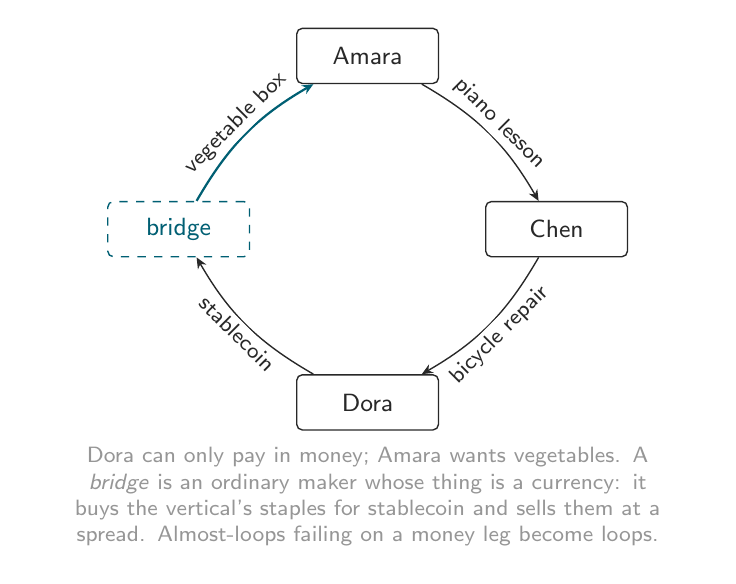
\begin{tikzpicture}
  \node[maker] (A) at (90:22mm) {Amara};
  \node[maker] (C) at (0:24mm) {Chen};
  \node[maker] (D) at (-90:22mm) {Dora};
  \node[maker, dashed, draw=accent, text=accent] (M) at (180:24mm) {bridge};
  \draw[flow] (A) to[bend left=15] node[lbl, sloped, above] {piano lesson} (C);
  \draw[flow] (C) to[bend left=15] node[lbl, sloped, below] {bicycle repair} (D);
  \draw[flow] (D) to[bend left=15] node[lbl, sloped, below] {stablecoin} (M);
  \draw[strong] (M) to[bend left=15] node[lbl, sloped, above] {vegetable box} (A);
  \node[note, text width=84mm] at (0,-34mm) {Dora can only pay in money; Amara wants vegetables. A \emph{bridge} is an ordinary maker whose thing is a currency: it buys the vertical's staples for stablecoin and sells them at a spread. Almost-loops failing on a money leg become loops.};
\end{tikzpicture}
\end{document}
